\section{Модель трехатомного гидрида с деформационной степенью свободы.}

Рассмотрим симметричные трехатомные гидриды $\ce{H2X}$. Они представляются хорошим объектом для изучения вращательной динамики и влияния колебательных движений на характер вращательного движения. В условиях высокого вращательного возбуждения легкие концевые атомы ставовятся подвижными, подвергаясь воздействию центробежных сил. Также, небольшое количество внутренних степеней свободы, делает эту систему доступной для изучения описанным методом. 

В качестве первой системы рассмотрим простейшую модель симметричной трехатомной молекулы $\ce{H2X}$. В качестве первого \underline{упрощения} зафиксируем расстояния между легкими атомами и центральным атомом. Таким образом, колебательная динамика молекулярной системы сводится к колебанию ножничного типа. Также, будем считать, что масса тяжелого центрального атома много больше масс легких атомов (\underline{фактически, бесконечность}), что позволит нам поместить центр масс молекулярной системы на тяжелый атом. Несмотря на кажущуюся примитивность описанной модели, она позволяет на качественном уровне описать колебательно-вращательное взаимодействие в трехатомных гидридах. Предложенная модель применима по той причине, что существенное влияние на колебательно-вращательное движение оказывает взаимодействие колебания деформационного типа с вращением молекулярной системы.

На рис.\eqref{fig:triatomic} молекула изображена в подвижной системе координат, причем ось $Ox$ параллельна биссектрисе валентного угла $q$, а ось $Oy$ перпендикулярна плоскости молекулы. Обозначим массу легких атомов -- $m$, расстояние между легким и тяжелым атомами -- $r_0$. 

\begin{figure}[!ht]
  \centering
	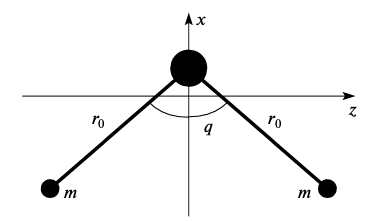
\includegraphics[width=0.4\textwidth]{../pictures/triatomic_fixed.png}
	\caption{Молекула $\ce{H2X}$ в подвижной системе отсчета.}
	\label{fig:triatomic}
\end{figure}

Выпишем координаты легких атомов в системе координат, связанной с центром масс.
\vverh
\begin{gather}
\left\{
\begin{aligned}
x_1 &= - r_0 \cos \lb \frac{q}{2} \rb \\
y_1 &= 0 \\
z_1 &= - r_0 \sin \lb \frac{q}{2} \rb 
\end{aligned}
\right. \quad \quad \quad
\left\{
\begin{aligned}
x_3 &= - r_0 \cos \lb \frac{q}{2} \rb \\
y_3 &= 0 \\
z_3 &= r_0 \sin \lb \frac{q}{2} \rb
\end{aligned}
\right.\notag
\end{gather}

Используя формулы, приведенные в предыдущей части, получим элементы матриц $\bba$, $\bbA$, $\bbI$, определяющих кинетическую энергию в форме Лагранжа в подвижной системе координат. Размер матрицы $\bba$ равен $\dim \bba = s \times s$, где $s$ - количество внутренних степеней свободы, т.е. в данном случае матрица $\bba$ является числом: $\bba = \frac{I_0}{2}$, где $I_0 = m r_0^2$. Несложные преобразования показывают, что матрица $\bbA$ является нулевой. Тензор инерции рассматриваемой системы имеет диагональный вид, причем компоненты $I_{xx}$, $I_{zz}$ в сумме дают $I_{yy}$ (т.к. система плоская): $I_{xx} = 2 I_0 \sin^2 \lb \frac{q}{2} \rb$, $I_{yy} = 2I_0$, $I_{zz} = 2I_0 \cos^2 \lb \frac{q}{2} \rb$. Итак, кинетическая энергия 
в форме Лагранжа принимает следующий вид:
\vverh
\begin{gather}
T_\mathcal{L} = \frac{1}{2} \sum_i m_i \dot{\vec{R}}_i^2 + \vec{\Omega}^{\, \top} \sum_i m_i \left[ \vec{R}_i \times \dot{\vec{R}}_i \right] + \frac{1}{2} \vec{\Omega}^{\, \top} \bbI \ \vec{\Omega} = \frac{1}{2} \frac{I_0}{2} \dot{q}^2 + \frac{1}{2} \vec{\Omega}^{\, \top} \bbI \ \vec{\Omega}. \notag
\end{gather} 

Для перехода к кинетической энергии в форме Гамильтона применим формулы, полученные при помощи подхода Фробениуса к обращению блочных матриц. Т.к. $\bbA = \bbzero$: $\bbG_{11} = \bbI^{-1}$, $G_{12} = G_{21} = \bbzero$, $\bbG_{22} = \bba^{-1}$. Обращая матрицу тензора инерции и раскрывая матричное выражение в скалярное, получаем кинетическую энергию в Гамильтоновском представлении:
\vverh
\begin{gather}
T_\mathcal{H} = \frac{1}{2} \lb \frac{J_x^2}{I_{xx}} + \frac{J_y^2}{I_{yy}} + \frac{J_z^2}{I_{zz}} \rb + \frac{p^2}{I_0}, \notag
\end{gather}

В качестве потенциала, описывающего деформационное колебание, был взят потенциал Пешля-Теллера: $V = \frac{1}{2I_0} \lb \frac{V_{-}}{1 - \cos q} + \frac{V_{+}}{1 + \cos q} \rb$, где постоянные $V_{-}$, $V_{+}$ могут быть найдены исходя из равновесного значения угловой координаты $q_0$ и гармонической частоты деформационного колебания $\omega_0$:
\vverh
\begin{gather}
V_{\pm} = \frac{1}{4} I_0^2 \omega_0^2 (1 \pm \cos q_0 )^2. \notag
\end{gather}

Выбор потенциала обусловлен тем, что задача описания энергетического спектра квантового осциллятора с потенциалом этого типа допускает точное аналитическое решение:
\vverh
\begin{gather}
E_n = \frac{1}{I_0} \hbar^2 \left[ n + \frac{1}{2 \hbar} \lb \sqrt{V_{-}} + \sqrt{V_{+}} \rb \right] \times \left[ n + 1 + \frac{1}{2 \hbar} \lb \sqrt{V_{-}} + \sqrt{V_{+}} \rb \right], \quad n = 0, 1, 2, \dots \notag 
\end{gather}

Также отметим, что аналитическая зависимость эффективного потенциала $V_{eff.}$ (получение и смысл, которого будут объяснены в следующей части) от координаты $q$ аналогичен зависимости потенциала $V(q)$. Следовательно квантовую колебательную задачу с потенциалом $V_{eff.}$ можно рассматривать, считая компоненты вектора углового момента $J_\alpha, \ \alpha = (x, y, z)$ параметрами. То есть, спектр собственных значений будет описываться формулой того же вида:
\vverh
\begin{gather}
E_n = \frac{1}{I_0} \hbar^2 \left[ n + \frac{1}{2 \hbar} \left( \sqrt{V_{-} + J_x^2} + \sqrt{V_{+} + J_z^2} \right) \right] \times \left[ n + 1 + \frac{1}{2 \hbar} \left( \sqrt{V_{-} + J_x^2} + \sqrt{V_{+} + J_z^2} \right) \right], \notag \\ 
 \hspace{11cm} n = 0, 1, 2 \dots \notag
\end{gather}

Таким образом, каждый из уровней энергии $E_n$ осциллятора, существовавших в отсутствие вращения, при наличии вращения превращается в полосу, ширина которой определяется диапазоном возможных направлений вектора углового момента при его фиксированной длине (рисунок \eqref{fig:vib_levels}).

\begin{figure}[H]
  \centering
	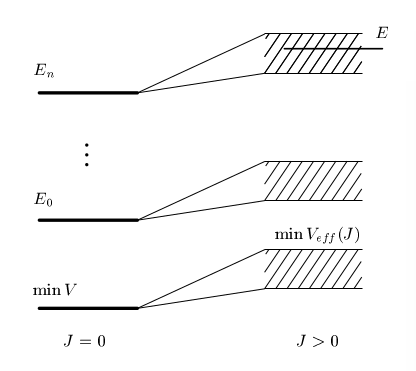
\includegraphics[width=0.5\textwidth]{../pictures/VibrationalLevels.png}
	\caption{Система колебательных уровней при отсутствии (слева) и при наличии (справа) вращения для одномерной задачи с потенциалом Пешля-Теллера.}
	\label{fig:vib_levels}
\end{figure}
	
\subsection{Концепция поверхности вращательной энергии.}

Концепция ПВЭ, впервые сформулированная Картером и Патерсоном [1], позволяет описать вращательную динамику молекул и связанную с ней природу квантовых вращательных спектров. ПВЭ представляет собой двумерную поверхность. Величина вращательной энергии откладывается в направлении вектора углового момента относительно молекулярно-фиксированной системы координат (при фиксированной длине вектора углового момента). Центросимметричность поверхности вращательной энергии является следствием наличия инверсии у вращательной задачи (изменение направления вращения системы приводит к обращению направления вектора углового момента, но сохраняет вращательную энергию). \\

Величина вращательной энергии определяется эффективным вращательным гамильтонианом, который может быть получен по следующей схеме. Рассмотрим компоненты вектора углового момента в качестве параметров в колебательно-вращательном гамильтониане $\mathcal{H} = \mathcal{H} (\vec{q}, \vec{p}, \vec{J})$. Определим равновесные значения обобщенных координат $\vec{q}_e = \vec{q}_e (\vec{J})$ и импульсов $\vec{p}_e = \vec{p}_e (\vec{J})$ как решения системы:
\begin{gather}
\left\{
\begin{aligned}
\lb \frac{\partial \mathcal{H}}{\partial \vec{q}} \rb_{\substack{\vec{q} = \vec{q}_e \\ \vec{p} = \vec{p}_e}} = \vec{0} \\
\lb \frac{\partial \mathcal{H}}{\partial \vec{p}} \rb_{\substack{\vec{q} = \vec{q}_e \\ \vec{p} = \vec{p}_e}} = \vec{0}
\end{aligned}
\right. \label{eff_ham}
\end{gather}

Эффективный вращательный гамильтониан получают заменяя обобщенные координаты $\vec{q}$ и сопряженные им импульсы $\vec{p}_e$ в колебательно-вращательном гамильтониане на их эффективные значения: $\mathcal{H}_r = \mathcal{H} (\vec{q}_e, \vec{p}_e, \vec{J})$.
Уравнения \eqref{eff_ham} могут быть рассмотрены с точки зрения модели ''мягкого тела''. При фиксированном направлении вектора углового момента внутренние координаты находятся в некотором новом равновесном состоянии, появившемся под действим центробежных сил. При этом внутримолекулярные колебания отсутствуют, и молекула вращается вокруг фиксированной в пространстве оси.
Между приближением Борна-Оппенгеймера и описанной процедурой можно провести определенные аналогии. В рамках первого приближения движения ядерной подсистемы принимают медленными по сравнениями с движениями электронной подсистемы, поэтому от суммарного гамильтониана системы переходят к электронному гамильтониану $\mathcal{H}_e$, параметрически зависящему от ядерных координат. В рамках описанной процедуры принимается, что самым медленным движением является вращение.
Второе векторное соотношение в системе \eqref{eff_ham} приводит к постоянству обобщенных координат: $\dot{\vec{q}} = 0$. Перепишем колебательно-вращательный гамильтониан в условиях $\vec{q} = \vec{q}_e$, $\vec{p} = \vec{p}_e$. Для этого получим выражение кинетической энергии в лагранжевых переменных $T_\mathcal{L} = T_\mathcal{L} (\vec{q}, \dot{\vec{q}} = \vec{0}, \vec{\Omega})$ и воспользуемся теоремой Донкина для перехода к гамильтоновым переменным:
\vverh
\begin{gather}
T_\mathcal{L}(\vec{q}, \dot{\vec{q}} = 0, \vec{\Omega}) = \frac{1}{2} \vec{\Omega}^{\, \top} \bbI \, \vec{\Omega} \quad \implies \quad T_\mathcal{H} = \frac{1}{2} \vec{J}^{\, \top} \bbI^{-1} \vec{J} \notag \\
\mathcal{H}(\vec{q}_e, \vec{p}_e, \vec{J}) = \frac{1}{2} \vec{J}^{\, \top} \bbI \, \vec{J} + V(\vec{q}_e) = V_{eff.} (\vec{q}_e, \vec{J}), \label{eff_ham2}
\end{gather}

\vlevo где $V_{eff.}$ -- эффективный потенциал. Соотношение \eqref{eff_ham2} позволяет получить зависимость $\vec{q}_e = \vec{q}_e (\vec{J})$, не решая систему \eqref{eff_ham}:
\begin{gather}
\lb \frac{\partial V_{eff.}}{\partial \vec{q}} \rb_{\vec{q} = \vec{q}_e} = \vec{0} \notag
\end{gather}

Т.к. построение поверхности вращательной энергии происходит при постоянном модуле вектора углового момента, то следует перейти к двум угловым переменным $\phi$, $\theta$, определяющим направление вектора углового момента. Таким образом уравнение ПВЭ принимает следующий вид: 
\vverh
\begin{gather}
E_r (\phi, \theta; J) = V_{eff.} (\vec{q}_e (\phi, \theta; J), \phi, \theta; J) \notag
\end{gather}

При анализе вращательной динамики сущесвенное значение имеют стационарные точки ПВЭ, их расположение на поверхности и их тип. Вследствие центросимметричности ПВЭ стационарные точки существуют в виде пар, эквивалентных относительно операции инверсии. Каждой паре симметрично расположенных точек соответствует одна ось, вокруг которой может вращаться вектор углового момнета. Устойчивость соответствующей оси зависит от типа стационарной точки: точки минимума и максимума порождают стабильные оси, а седловидные точки -- нестабильные. Положение стационарных точек может быть установлено при решении следующей системы уравнений:
\vverh
\begin{gather}
\left\{
\begin{aligned}
\frac{\partial E_r}{\partial \phi} = \frac{\partial V_{eff.}}{\partial \phi} + \frac{\partial V_{eff.}}{\partial \vec{q}_e} \frac{\partial \vec{q}_e}{\partial \phi} = 0 \\
\frac{\partial E_r}{\partial \theta} = \frac{\partial V_{eff.}}{\partial \theta} + \frac{\partial V_{eff.}}{\partial \vec{q}_e} \frac{\partial \vec{q}_e}{\partial \theta} = 0
\end{aligned}
\right. \notag
\end{gather}

Для определения типа стационарной точки необходимо исследовать знакоопределенность гессиана в окрестности исследуемой точки: 
\vverh
\begin{gather}
\mathds{H} = \begin{pmatrix}
\partial^2 E_r / \partial \phi^2 (\phi_s, \theta_s) & \partial^2 E_r / \partial \phi \partial \theta (\phi_s, \theta_s) \\
\partial^2 E_r / \partial \theta \partial \phi (\phi_s, \theta_s) & \partial^2 E_r / \partial \phi^2 (\phi_s, \theta_s)
\end{pmatrix}, \notag
\end{gather}
\vlevo где $(\phi_s, \theta_s)$ -- углы, определяющие положение рассматриваемой стационарной точки.

\subsection{Получение ПВЭ модельной системы.}

Построим эффективный гамильтониан исходя из колебательно-вращательного гамильтониана для модельной системы. 
\vverh
\begin{gather}
H(\vec{q}, \vec{p}, \vec{J}) = \frac{1}{2I_0} \left[ \frac{J_x^2 + V_{-}}{1-\cos q} + \frac{J_z^2 + V_{+}}{1 + \cos q} + \frac{J_y^2}{2} \right] + \frac{p^2}{I_0} \label{model_ham}
\end{gather}

Решение уравнений \eqref{eff_ham} дает нам выражения эффективных обобщенных координат и импульсов:
\begin{gather}
\left\{
\begin{aligned}
\cos q_e &= \frac{\sqrt{A_{+}} - \sqrt{A_{-}}}{\sqrt{A_{+}} + \sqrt{A_{-}}} \\
p_e &= 0,
\end{aligned}
\right.
\label{eq_angle}
\end{gather}

\vlevo где $A_{+} = J_z^2 + V_{+}$, $A_{-} = J_x^2 + V_{-}$. 
Полученное выражение позволяет построить зависимость равновесного значения межсвязевого угла $q_e$ от модуля вектора углового момента $J$. 
\vverh
\begin{figure}[!ht]
  \centering
	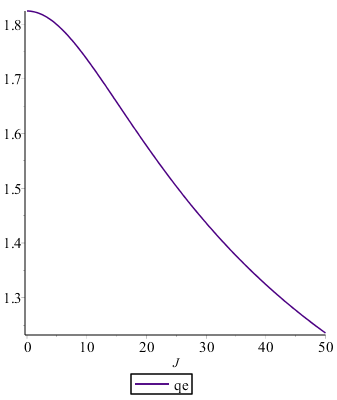
\includegraphics[width=\textwidth]{../pictures/qe_rigid.png}
	\caption{Зависимость равновесного значения $q_e$ от модуля вектора углового момента $J$.}
	\label{fig:qe}
\end{figure}

Подставляем выражения эффективных координаты $q_e$ и импульса $p_e$ в гамильтониан \eqref{model_ham}, выполняя несложные алгебраические преобразования, приходим к следующему виду эффективного гамильтониана:
\vverh
\begin{gather}
H_r = \frac{1}{4I_0} \left[ \left( \sqrt{A_{+}} + \sqrt{A_{-}} \right)^2 + J_y^2 \right] \notag \\
E_r (\phi, \theta; J) = \frac{1}{4I_0} \left[ \left( \sqrt{V_{+} + J^2 \cos^2 \theta} + \sqrt{V_{-} + J^2 \cos^2 \phi \sin^2 \theta} \right)^2 + J^2 \sin^2 \phi \sin^2 \theta \right] \notag
\end{gather}

\begin{figure}[H]
  \centering
	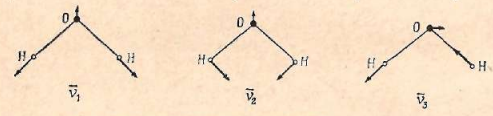
\includegraphics[scale=0.75]{../pictures/NormalModes.png}
	\caption{Форма нормальных колебаний молекулы воды.}
\end{figure}

\begin{figure}[H]
\begin{tabular}{|*7{c|}}  \hline
\rule[-2ex]{0pt}{6ex} & $\angle$ H-NonMe-H & $r_{e, NonMe-H}$, \AA & $\nu_1$, см$^{-1}$ & $\nu_2$, см$^{-1}$ & $\nu_3$, см$^{-1}$ & $\nu_{av.}$, см$^{-1}$  \\ \hline
\rule[-2ex]{0pt}{6ex} $\ce{H2O}$ & $104^\circ 31^{'}$ & $0,95718 \pm 0,0003$ & 3656,65 & 1594,78 & 3755,79 & 3706,22 \\ \hline
\rule[-2ex]{0pt}{6ex} $\ce{H2S}$ & $92^\circ 06^{'}$ & 1,3362 & 2614,56 & 1182,68 & 2625 & 2619,78 \\ \hline
\rule[-2ex]{0pt}{6ex} $\ce{H2Se}$ & $90^\circ 55^{'}$ & $1,460 \pm 0,03$ & 2344,50 & 1034,21 & 2357,80 & 2351,15 \\ \hline
\rule[-2ex]{0pt}{6ex} $\ce{H2Te}$ & $90^\circ 15^{'}$ & 1,658 & (2000) & 860,765 & (2000) & (2000) \\ \hline
\end{tabular}
\caption{Справочные данные по трехатомным гидридам.}
\label{table1}
\end{figure}

Построим несколько поверхностей вращательной энергии для молекулы $\ce{H2O}$ при разных значениях модуля вектора углового момента. 

\begin{figure}[H]
  \centering
	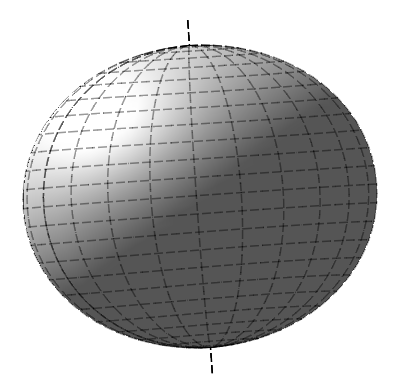
\includegraphics[width=0.25\textwidth]{../pictures/Rigid_RES_10.png}
	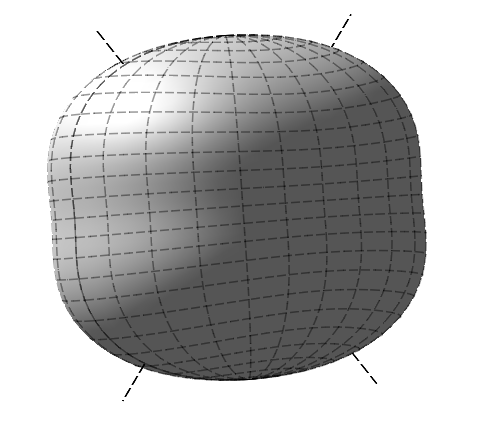
\includegraphics[width=0.3\textwidth]{../pictures/Rigid_RES_30.png}
	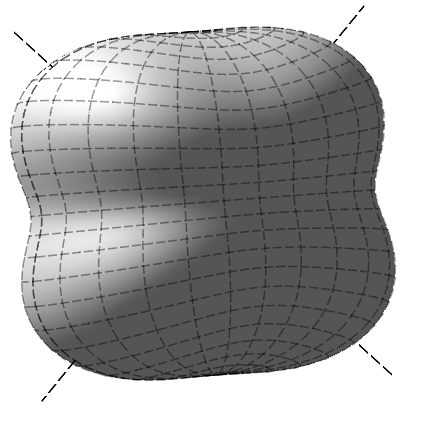
\includegraphics[width=0.3\textwidth]{../pictures/Rigid_RES_50.png}
	\caption{Перестройка поверхности вращательной энергии $\ce{H2O}$ при увеличении модуля вектора углового момента $J=10, 30, 50$.}
	\label{fig:triatomic}
\end{figure}

Несложно показать, что при малых значениях момента ПВЭ имеет две устойчивых оси вращения $Oz$ и $Oy$ и одну неустойчивую ось, проходящую через пару симметричных седловых точек. Таким образом, на ПВЭ имеется два типа прецессионных движений вектора углового момента -- вокруг оси $Oz$ (им соответствуют квантовые уровни в верхней части вращательного мультиплета) и вокруг оси $Oy$ (им соответствуют квантовые уровни в нижней части вращательного мультиплета). Анализ стационарных точек показывает, что перестройка ПВЭ наступает при достижении критического значения модуля углового момента:
\vverh
\begin{gather}
J_{cr.} = \sqrt{V_{-} - V_{+}} = I_0 \omega_0 \sqrt{|\cos q_0|} \label{critical_moment}
\end{gather}

При перестройки поверхности две точки максимума теряют свою устойчивость и становятся седловыми точками, в то время как возникают четыре новых точки максимума с координатами $(\theta_e, 0), (\theta_e, \pi), (\pi - \theta_e, 0), (\pi - \theta_e, \pi)$, где $\theta_e =\frac{1}{2} \arcsin \lb \frac{V_{-} - V_{+}}{J^2} \rb $. 